\section{System Overview}
\label{sec:fdsp-tpcelec-overview}

The TPC electronics encompass the hardware systems necessary to 
amplify, digitize, and transmit the \dword{tpc} ionization charge 
signals out of the \dword{dune} \dword{sp} \dword{detmodule}. This 
includes the cryogenic front-end electronics (amplifiers, digitizers, 
digital controllers), power and data cabling and their cryostat 
feedthroughs, external (non-cryogenic) digital control electronics and 
power supplies, in addition to the system providing the bias voltage
to the \dwords{apa}.  The TPC electronics as presented here does not 
include the electronics associated with the detection 
and recording of \dword{lar} scintillation photons, nor the \dword{daq} 
computing systems needed to capture and record these data.

The main difference between the \dword{dune} \dword{sp} \dword{detmodule} 
and previous experiments or prototypes using \dword{lar} technology is
that for the first time all the signal processing for the readout of the
wires of the \dwords{apa} takes place inside the \dword{lar}, in boards that 
are directly mounted on the \dword{apa}. This approach to the \dword{tpc}
readout has been tested for the first time in the \dword{pdsp} prototype,
and is also being adopted by the \dword{sbnd} experiment. Sometimes, the 
\dword{tpc} readout components immersed in the \dword{lar} are referred 
to as the \dword{ce}. 

The electronics are mounted inside the \dword{lar} to exploit the fact that 
charge carrier mobility in silicon is higher, and thermal fluctuations are lower,  
at \dword{lar} temperature than at room temperature. For \dword{cmos} 
electronics, this results in substantially higher gain and lower noise 
at \dword{lar} temperature than at room temperature~\cite{DeGeronimo:2011zz}.
Mounting the \dword{fe} electronics on the \dword{apa} frames also minimizes 
the input capacitance, which further contributes to the noise reduction.  
Furthermore, placing the digitizing and multiplexing electronics inside 
the cryostat reduces the total number of penetrations into the cryostat 
and minimizes the number of cables coming out of it.

As the full \dword{tpc} electronics chain for the \dword{spmod} includes 
many components on the warm side of the cryostat as well, the \dword{dune} 
consortium designated to develop this system is formally called 
the \dword{dune} \dword{sp} \dword{tpc} electronics consortium.

This overview section starts with a review of the considerations that
have led to the proposed design for the \dword{dune} \dword{sp} detector, 
then discusses how the detector requirements follow from the physics goals 
of the experiment. The reader will find a detailed description of all the 
\dword{tpc} electronics detector components in Section \ref{sec:fdsp-tpcelec-design},
including a discussion of how the lessons learned from the construction,
integration, installation and commissioning of \dword{pdsp} have informed
the design of the \dword{dune} \dword{sp} module and how the early data
from \dword{pdsp} validate this design. The description of the detector
design is then followed by discussions 
of the \dword{qa} program and the plans for production and assembly, 
and for integration, installation and commissioning, in 
Sections~\ref{sec:fdsp-tpcelec-qa}--\ref{sec:fdsp-tpcelec-integration}. 
Section~\ref{sec:fdsp-tpcelec-interfaces} discusses the interfaces with 
detector components provided by other consortia, with \dword{tc}, and with the physics group. 
Sections~\ref{sec:fdsp-tpcelec-safety}--\ref{sec:fdsp-tpcelec-management} 
conclude the chapter with plans for addressing safety issues and risks during the
construction, installation, and operation of the detector, and 
an outline of the organization of the \dword{tpc} electronics consortium, 
with a timeline for the \dword{detmodule} construction and an estimate
of the resources required.

%%%%%%%%%%%%%%%%%%%%%%%%%%%%%%%%%%%
\subsection{Introduction}
\label{sec:fdsp-tpcelec-overview-intro}

In the \dword{dune} \dword{spmod} a \dword{mip} deposits on average between
\SI{20}{k}{e$^-$} and \SI{30}{k}{e$^-$} on each collection wire, assuming a drift \efield
of \spmaxfield and an electron lifetime of \SI{6}{ms}, as discussed in
Chapter~\ref{ch:fdsp-execsum}, and assuming full transparency during the 
electron transport through the grid plane and the two planes of induction
wires, as discussed in Chapter~\ref{ch:fdsp-apa}. The larger of the two numbers 
is for \dwords{mip} close to the anode plane, and the smaller
takes into account the electron capture by electronegative impurities during the electron
drift tracks close to the cathode plane. 

The \dword{dune} \dword{sp} \dword{tpc} is a unit-gain device where the 
electrical signal is produced by the drift of the charges near the wires, 
in contrast to signal production in gaseous wire 
chambers, where the \efield is strong enough to provide additional
ionization and signal multiplication. The signal induced in the \dword{dune}
\dword{spmod} wires is bipolar on the induction wires, negative when the
electrons drift toward the wires, and positive when they drift away from
the wires. On the collection wires signals are unipolar (negative).
The signal duration is of the order of microseconds, and tends to be narrower
for the collection plane due to the enhancement of the weighting field for
the collection wires. Due to the lack of amplification of electrons inside 
\dword{lar}, low noise is essential for the \dword{ce} to reliably extract the 
ionization electron signal from both the collection and induction wire planes 
in a \dword{sp} \dword{lartpc}. 

The reduction in noise level obtained with the \dword{fe} electronics at 
\dword{lar} temperature greatly extends the reach of the \dword{dune} 
physics program. It allows measurement of smaller charge deposits, which 
mitigates against the risk of inability to reach the desired drift field 
or a lower electron lifetime than desired due to electronegative impurities.
For example, given an electron lifetime of \SI{3}{ms} and a drift \efield
of \SI{0.25}{kV/cm}, the charge deposited in the collection wires from a 
\dword{mip} close to the cathode plane is reduced to \SI{10}{k}{e$^-$}.
The exact requirement of the minimal \dword{s/n} required for pattern
recognition depends on the tracking algorithms and the offline signal 
processing. For the design of the \dword{tpc} electronics we use the
minimal requirement of a total \dword{enc} of less than 1000 e$^-$, consistent 
with a \dword{s/n} of at least 10 on the collection wires, even in the
pessimistic case where the electron lifetime and the \efield just meet 
the required design values discussed in Chapter~\ref{ch:sp-hv}. Considering
the difference in signal amplitudes between collection and induction wires
and the bipolar shape of the signal on the latter, this requirement corresponds 
to a \dword{s/n} of at least 5 on the induction wires. This asymmetric requirement 
for the minimal \dword{s/n} on the collection and induction wires has already been 
adopted by the \dword{sbnd} experiment~\cite{bib:sbnddoc1921}.

The goal is to keep the total noise level as low as possible. For example, an 
increase in the \dword{s/n} above 15 allows the observation of MeV-scale photons, 
as recently demonstrated by \dword{argoneut}~\cite{Acciarri:2018myr}. This enables  
reconstruction of both photons released during de-excitation of the nucleus and 
part of the energy transferred to final-state neutrons. Low noise is also crucial
for the baseline oscillation analysis described in Chapter 5 of Volume~\volnumberphysics{} 
of this \dword{tdr}, \voltitlephysics{}. The event classification is based
on a \dword{cvn} that uses as inputs three images of the neutrino interactions, 
one for each of the three readout views, using the reconstructed hits on the 
individual wire planes. This approach relies on low noise levels. Decreasing 
the noise level also increases the reach of low-energy physics measurements 
like those associated with stellar core-collapse \dword{snb}. 
Finally, a low noise level opens up the possibility of using $\mathrm{{}^{39}Ar}$ 
beta decays to calibrate the \dword{dune} \dword{spmod}~\cite{MICROBOONE-NOTE-1050-PUB}.
Instead of zero suppression, the \dword{dune} \dword{daq} system uses lossless 
data compression, as discussed in Section~\ref{sec:fd-daq:requirements}, that
becomes more efficient as the noise level is reduced. Therefore, the noise level 
also affects the bandwidth requirements for the \dword{daq} system,
discussed in Chapter~\ref{ch:sp-daq};
these bandwidth requirements can be a limiting factor for low-energy
physics signals, particularly those of astrophysical origin.

\begin{dunefigure}
[The baseline architecture for the TPC electronics.]
{fig:ce-scheme}
{The baseline architecture for the \dword{tpc} electronics. The basic unit is the
128-channel \dword{femb}. The scheme includes also the
\dwords{sipm} used for the readout of the \dwords{pd}.}
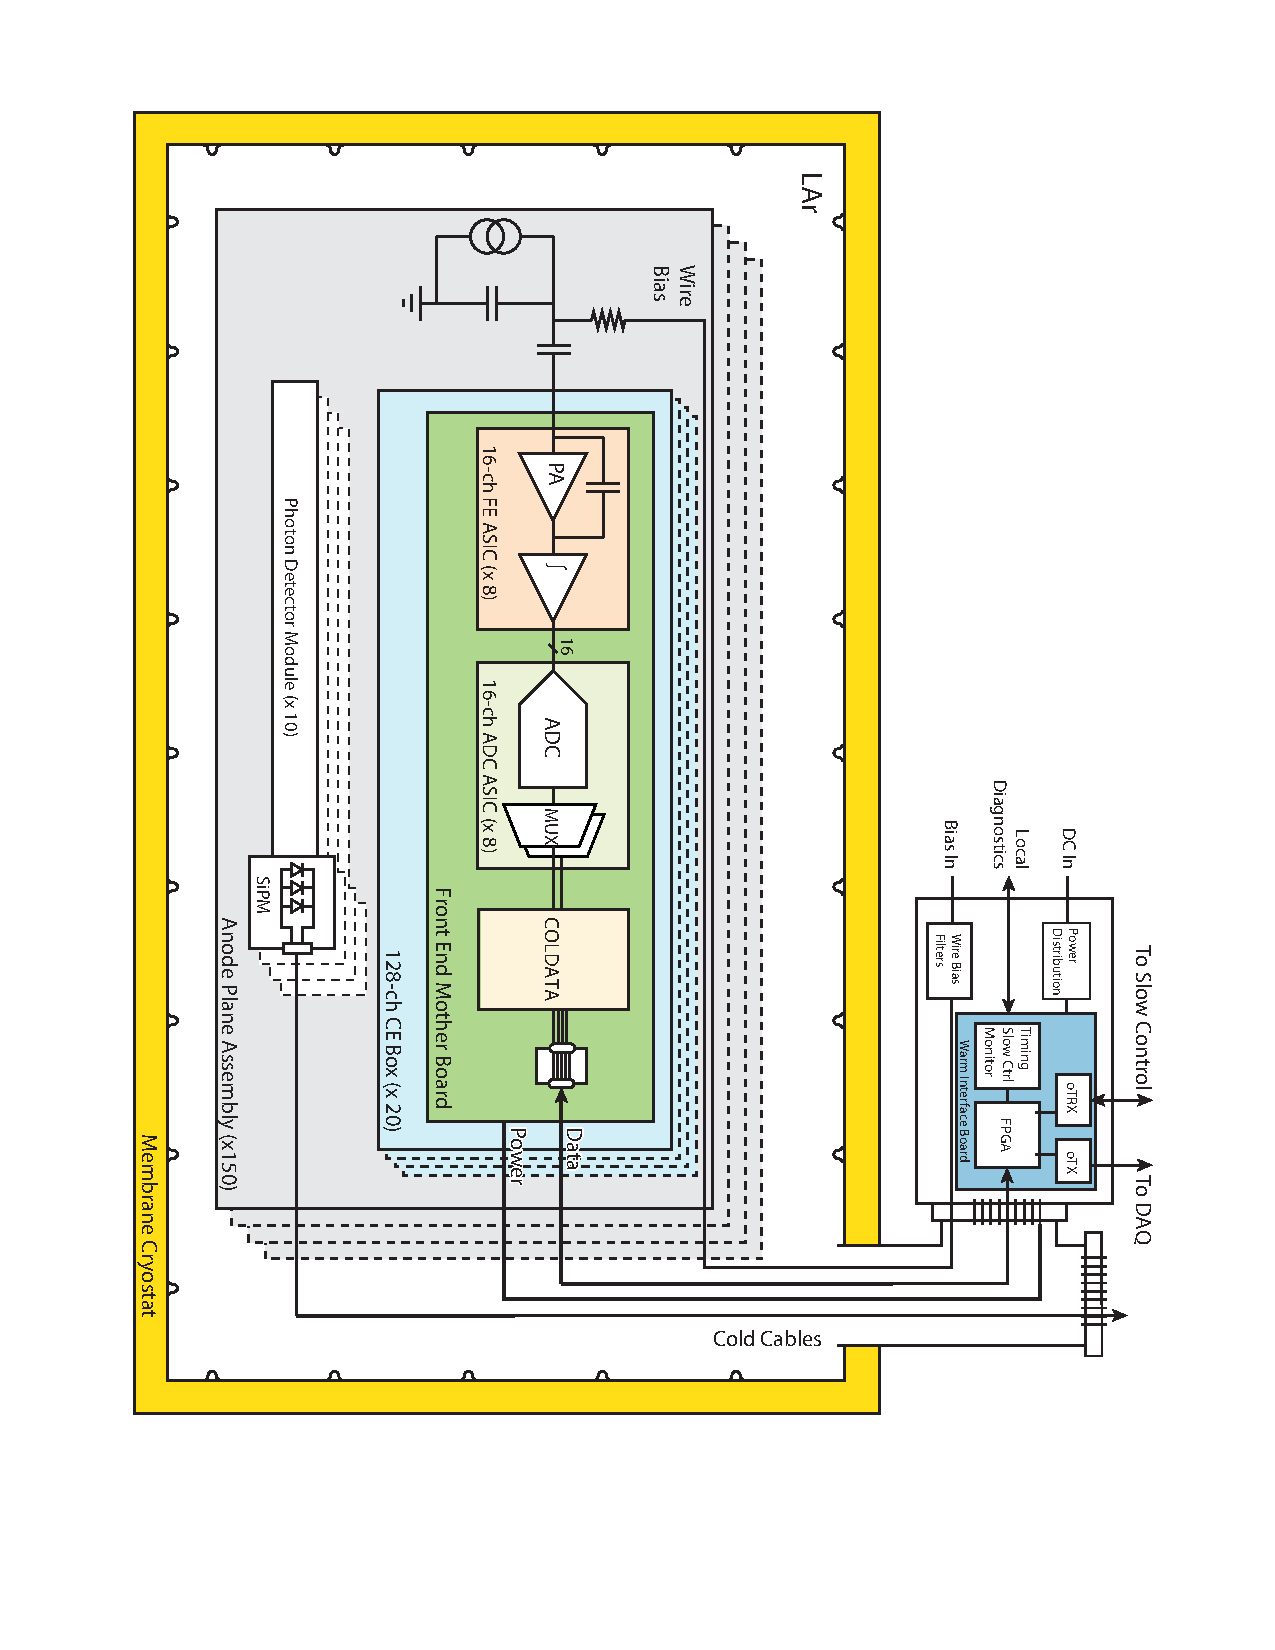
\includegraphics[width=0.99\linewidth]{sp-tpcelec-schematic-v3.pdf}
\end{dunefigure}

To retain maximum flexibility in optimizing reconstruction algorithms after 
the \dword{dune} data is collected, the \dword{tpc} electronics are designed 
to produce a digital record representing the waveform of the current produced 
by charge collection and induction on the anode wires. Each anode wire signal is 
input to a charge-sensitive amplifier, followed by a pulse-shaping circuit and 
an \dword{adc}. To minimize the number of cables and cryostat penetrations, 
the \dwords{adc} as well as the amplifier/shapers are located in the \dword{lar}, 
and digitized data from many wires merge onto a much smaller set of high-speed 
serial links. The \dword{tpc} signal processing is implemented in \dfirsts{asic}
using \dword{cmos} technology. The \dword{tpc} is continuously read out, resulting 
in a digitized \dword{adc} sample from each \dword{apa} channel (wire). The 
\dwords{asic} used for the readout of the \num{2560} wires of each \dword{apa} 
are mounted on \dfirsts{femb}, as shown in Figure~\ref{fig:ce-scheme}. These are
connected to \dwords{wib} located outside of the cryostat via the \dword{ce} signal 
cable flange located at the \dword{ce} \fdth at the top of the cryostat.
The \dwords{wib} are installed, together with \dword{ptc} that distribute
the power and the clock and control signals, in a \dword{wiec} that is
mounted on the signal flange. From the \dwords{wib} the data is sent to 
the \dword{daq} back-end on an optical fiber network, as discussed in 
Chapter~\ref{ch:sp-daq}. 

\subsection{Requirements and Specification}
\label{sec:fdsp-tpcelec-overview-requirements}

A number of specifications are imposed on the \dword{tpc} electronics in addition to the 
noise requirement (\dword{enc}~$<\SI{1000}{e^-}$). Some of them, labeled as 
SP-FD in Table~\ref{tab:specs:SP-ELEC}, are derived from \dword{dune}'s 
overall physics goals. The rest, labeled as SP-TPC, are engineering specifications 
derived from the design choices for the \dword{ce}. Note that requirements 
SP-FD-01, SP-FD-03, SP-FD-04, and SP-FD-05 do not apply to the \dword{tpc} electronics. 

\fixme{Marco: the LBNC and every reader complain about the presence of
requirements SP-FD-01, SP-FD-03, SP-FD-04, and SP-FD-05. And I hate the
blank space on this page.}

\pagebreak
% This file is generated, any edits may be lost.
\begin{footnotesize}
%\begin{longtable}{p{0.14\textwidth}p{0.13\textwidth}p{0.18\textwidth}p{0.22\textwidth}p{0.20\textwidth}}
\begin{longtable}{p{0.12\textwidth}p{0.18\textwidth}p{0.17\textwidth}p{0.25\textwidth}p{0.16\textwidth}}
\caption{Specifications for SP-ELEC \fixmehl{ref \texttt{tab:spec:SP-ELEC}}} \\
  \rowcolor{dunesky}
       Label & Description  & Specification \newline (Goal) & Rationale & Validation \\  \colhline

   
  \newtag{SP-FD-2}{ spec:system-noise }  & System noise  &  $<\,\SI{1000}\,e^-$ &  Provides $>$5:1 S/N on induction planes for  pattern recognition and two-track separation. &  ProtoDUNE and simulation \\ \colhline
    
    
   \newtag{SP-FD-13}{ spec:fe-peak-time }  & Front-end peaking time  &  \SI{1}{\micro\second} \newline ( Adjustable so as to see saturation in less than \SI{10}{\%} of beam-produced events ) &  Vertex resolution; optimized for \SI{5}{mm} wire spacing. &  ProtoDUNE and simulation \\ \colhline
    
   
  \newtag{SP-FD-14}{ spec:sp-signal-saturation }  & Signal saturation level  &  \num{500000} electrons &  Maintain calorimetric performance for multi-proton final state. &  Simulation \\ \colhline
    
    
   
  \newtag{SP-FD-19}{ spec:adc-sampling-freq }  & ADC sampling frequency  &  $\sim\,\SI{2}{\mega\hertz}$ &  Match \SI{1}{\micro\second} shaping time. &  Nyquist requirement and design choice \\ \colhline
    
    
   \newtag{SP-FD-20}{ spec:adc-number-of-bits }  & Number of ADC bits  &  \num{12} bits \newline ( \num{13} bits ) &  ADC noise contribution negligible (low end); match signal saturation specification (high end). &  Engineering calculation and design choice \\ \colhline
    
   
  \newtag{SP-FD-21}{ spec:ce-power-consumption }  & Cold electronics power consumption   &  $<\,\SI{50}{ mW/channel} $ &  No bubbles in LAr to redice HV discharge risk. &  ProtoDUNE \\ \colhline
    
   
  \newtag{SP-FD-25}{ spec:non-fe-noise }  & Non-FE noise contributions  &  $<<\,\SI{1000}{enc} $ &  High S/N for high reconstruction efficiency. &  Engineering calculation and ProtoDUNE \\ \colhline
    
    
   
  \newtag{SP-FD-28}{ spec:dead-channels }  & Dead channels  &  $<\,\SI{1}{\%}$ &  Contingency for possible efficiency loss for $>\,$20 year operation.  &  ProtoDUNE \\ \colhline
    

   \newtag{SP-ELEC-1}{ spec:num-FE-baselines }  & Number of baselines in the front-end amplifier  &  2.0 \newline ( 2.0 ) &  Use a single type of amplifier for both induction and collection wires &  ProtoDUNE \\ \colhline
    
   \newtag{SP-ELEC-2}{ spec:gain-FE-amplifier }  & Gain of the front-end amplifier  &  $\sim\SI{20}{mV/fC}$ \newline (Adjustable in the range \SIrange{5}{25}{mV/fC}) &  The gain of the FE amplifier is obtained from the maximum charge to be observed without saturation and from the operating voltage of the amplifier, that depends on the technology choice. &   \\ \colhline
    
   \newtag{SP-ELEC-3}{ spec:syncronization-CE }  & System synchronization  &  \SI{50}{ns} \newline ( \SI{10}{ns} ) &  The dispersion of the sampling times on different wires of the APA should be much smaller than the sampling time (500 ns) and give a negligible contribution to the hit resolution. &   \\ \colhline
    
   
  \newtag{SP-ELEC-4}{ spec:num-channels-FEMB }  & Number of channels per front-end motherboard  &   &  The total number of wires on one side of an APA, 1,280, must be an integer multiple of the number of channels on the FEMBs. &  Design \\ \colhline
    
   \newtag{SP-ELEC-5}{ spec:FEMB-data-link }  & Number of links between the FEMB and the WIB  &  \num{4} at \SI{1.28}{Gbps} \newline ( \num{2} at \SI{2.56}{Gbps} ) &  Balance between reducing the number of links and reliability and power issues when increasing the data transmission speed. &  ProtoDUNE, Laboratory measurements on bit error rates \\ \colhline
    
   
  \newtag{SP-ELEC-6}{ spec:cold-cables-xsec }  & Cross section of cold cables  &  \SI{2.5}{inches} &  Avoid the need for further changes to the APA frame and for routing the cables along the cryostat walls &  Tests on APA frame prototypes \\ \colhline
    
   
  \newtag{SP-ELEC-7}{ spec:WIB-data-link }  & Data transmission speed between the WIB and the DAQ backend  &  \SI{10}{Gbps} &  Balance between cost and reduction of the number of optical fiber links for each WIB. &  ProtoDUNE, Laboratory measurements on bit error rates \\ \colhline
    
   
  \newtag{SP-ELEC-8}{ spec:cold-cables-xsec }  & Maximum diameter of conduit enclosing the cold cables while they are routed through the APA frame  &  \SI{6.35}{cm} (2.5") &  Avoid the need for further changes to the APA frame and for routing the cables along the cryostat walls &  Tests on APA frame prototypes \\ \colhline
    


\label{tab:specs:SP-ELEC}
\end{longtable}
\end{footnotesize}

\begin{itemize}
\item SP-FD-13: The \dword{fe} peaking time must be in the range \numrange{1}{3}\,\si{\micro\second} 
to match the time required for the drifting charges to travel from one plane of anode
wires to the next, which corresponds to the typical duration of the signal observed
on the wires. The planes of anode wires are separated by \SI{4.75}{mm} 
(see Chapter~\ref{ch:fdsp-apa}), and the drift velocity for the \efield{}s 
considered for \dword{dune} is in the range \SIrange{1.25}{1.5}{mm/$\mu$s}. 
A \dword{fe} peaking time  similar to the typical signal duration improves the 
detector's two-track resolution.  

\item SP-FD-14: The system must have a linear response up to an impulse input of 
at least \num{500000}\,$e^{-}$.  This corresponds roughly to the largest 
ionization signals expected. These occur in events where multiple protons are produced 
in the primary event vertex, in particular, when the trajectories of one 
or more of the protons are parallel to the wire, 
leading to collection of charge over a long path length within a short time.

\item SP-FD-19:  The \dword{adc} sampling frequency must be \SI{{\sim}2}{MHz},
This value is chosen to match a \dword{fe} shaping time of \SI{1}{\micro\second} 
(approximate Nyquist condition) while minimizing the data rate.

\item SP-FD-20: The \dword{adc} must digitize the charge deposited on the wires 
with 12~bits of precision.  The lower end of the \dword{adc} dynamic 
range is driven by the requirement that the digitization not contribute 
to the total electronics noise, as defined by requirement SP-FD-25. The upper end
is defined by SP-FD-14. Combining this with SP-FD-02 on the total electronics noise 
results in the need for 12~bits digitization. 

\item SP-FD-21: Preliminary studies indicate that the power dissipated by the 
electronics located in the \dword{lar} should be less than \SI{50}{mW/channel}. 
Lower power dissipation is desirable because the mass of the power cables scales 
with power. Ongoing studies focus on whether the amount of power dissipated by 
the electronics should be minimized further because of potential complications from 
argon boiling. 

\item SP-FD-25: 
The components of the readout chain, including the \dword{adc}
and the bias voltage supplies, together must not contribute significantly to
the overall noise. The \dword{adc} specifications for non-linearity and 
noise will depend on the gain of the \dword{fe}.

\item SP-FD-28: The fraction of non-functioning channels over 
\dword{dune}'s nominal \dunelifetime lifetime must not exceed 1\%. 
Ongoing studies will quantify the effect of failures
in the \dword{tpc} and electronics, including
single wire failures, and failures of groups of
\num{16}, \num{64}, or \num{128} channels.

\item SP-ELEC-1: The \dword{fe} must have an adjustable baseline such that a single
amplifier can process both the bipolar signal from the induction wires and the mostly 
unipolar signal from the collection wires. 

\item SP-ELEC-2: The \dword{fe} must have a gain that allows using the entire
voltage range provided by the chosen chip fabrication technology and operating
voltage without saturation for physics signals up to those specified in
SP-FD-14. Multiple gain settings could be made available to allow for optimization
of the detector performance.

\item SP-ELEC-3: The dispersion of the sampling times on the different wires of
all the \dwords{apa} in one \dword{dune} \dword{sp} detector module should
be less than \SI{50}{ns}. This value is much smaller than the 
time difference between to subsequent samples on the same wire
as defined by the sampling frequency (SP-FD-19) such that it gives
a negligible contribution to the single hit resolution (assuming
a drift velocity of \SI{1.6}{mm/$\mu$s}, the requirement of \SI{50}{ns}
corresponds to a contribution to the single hit resolution of \SI{80}{$\mu$m}).

\item SP-ELEC-4: The readout electronics for the \dword{apa} wires must be organized
into \dwords{femb} containing 128 channels. This number is a sub-multiple
of the number of wires on an \dword{apa} and is determined
by geometrical considerations, e.g., the number, size, and form
factor of the \dword{cr} boards introduced in Section~\ref{sec:fdsp-tpcelec-design-bias}.

\item SP-ELEC-5: The data from the \dwords{femb} must be transmitted to the
\dwords{wib} on a maximum of four links per board, each with a maximum
speed of \SI{1.28}{Gbps}, to minimize
the number of connections on the cryostat penetrations. This 
requires data transmission at high speeds, which 
increases the power consumption inside the \dword{lar}.
A reduction in the number of links per \dword{femb} to two
(with a link speed of \SI{2.56}{Gbps}) will be investigated.

\item SP-ELEC-6: Each \dword{wib} must read out four \dwords{femb}. This number
is chosen to balance the complexity of the boards, the mechanics
of the \dword{wiec} that houses the \dwords{wib}, and the 
required processing power in the \dword{fpga} inside the
\dword{wib}.

\item SP-ELEC-7: Each \dword{wib} must transmit data to the \dword{daq}
backend on optical links at a speed of $\sim\,\SI{10}{Gbps}$. This speed 
is a compromise between the cost of optical transmitters and
receivers and the complexity of the readout fiber plant.

\item SP-ELEC-8: All the cables required to provide the low-voltage power
and the control and readout for the \dwords{femb} mounted on
the bottom \dword{apa}, plus the bias voltage cables for
the same \dword{apa}, must fit inside two conduits with a
diameter of \SI{6.35}{cm} (2.5") that are inserted in the frame of
the \dword{apa}, as discussed in Section~\ref{sec:fdsp-tpcelec-interfaces-apa}. 
\end{itemize}

%%%%%%%%%%%%%%%%%%%%%%%%%%%%%%%%%%%
\subsection{Design}
\label{sec:fdsp-tpcelec-overview-design}

The baseline design of the \dword{tpc} electronics detector components is
based on the specifications presented in Section~\ref{sec:fdsp-tpcelec-overview-requirements}. 
Each individual \dword{apa} has \num{2560} channels read out by \num{20} 
\dfirsts{femb}, with each \dshort{femb} enabling digitized wire readout 
from \num{128} channels. One cable bundle connects each \dshort{femb} to
the outside of the cryostat via a \dword{ce} signal cable flange located 
at the \dword{ce} \fdth at the top of the cryostat, where a single flange 
services each \dword{apa}, as shown in Figure~\ref{fig:connections}. 
Two \dword{ce} signal flanges are on each \fdth and together account for 
all electronics channels associated with a pair of \dword{apa}s (upper 
and lower, vertically arranged). Each cable bundle contains wires for 
low-voltage (\dword{lv}) power, high-speed data readout, and clock or 
digital-control signal distribution. Eight separate cables carry the 
\dword{tpc} wire bias voltages from the signal flange to the \dword{apa} 
wire bias boards, in addition to the bias voltages for the field cage 
termination electrodes and for the electron diverters. An additional 
flange on the top of each \fdth services the \dword{pds} cables associated 
with the \dword{apa} pair. Low voltage power supplies and bias voltage
power supplies are located on the top of the cryostat. 

\begin{dunefigure}
[Connections between the signal flanges and \dword{apa}]
{fig:connections}
{Connections between the signal flanges and \dword{apa}. The lower 
\dword{apa} shares the photon detector flange with the 
upper \dword{apa} but has a separate TPC readout flange.}
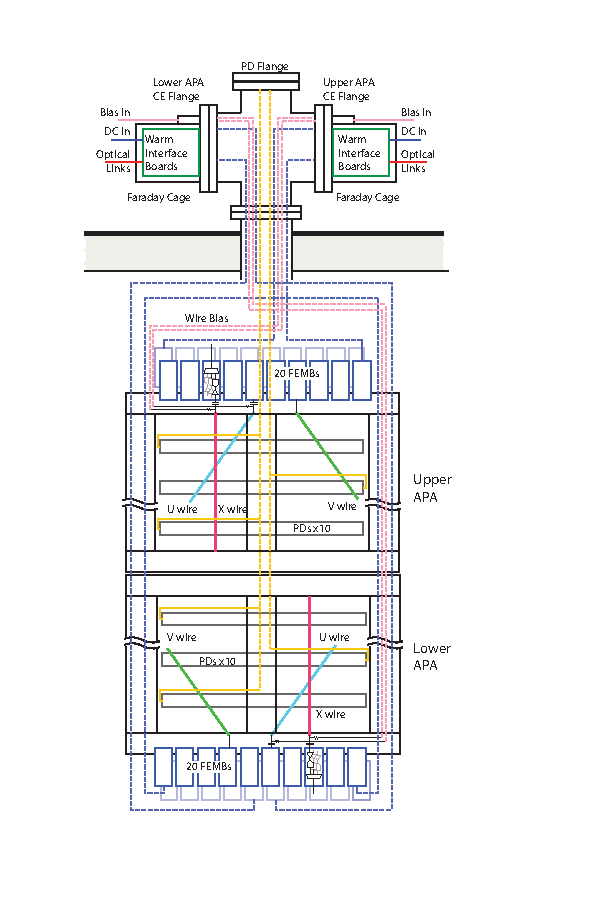
\includegraphics[width=0.7\textwidth]{sp-tpcelec-DUNE-FD-APA-readout-scheme-v1.pdf}
\end{dunefigure}

The baseline design for the \dword{spmod} \dword{tpc} electronics (the \dword{ce}) calls for three 
types of custom \dwords{asic} inside  the \dword{lar}:
\begin{itemize}
\item{a \num{16}-channel \dword{fe} \dword{asic} for amplification 
and pulse shaping (referred to as \dword{larasic});}
\item{a \num{16}-channel \num{12}-bit \dword{adc} \dword{asic} 
operating at \SI{{\sim}2}{MHz} (referred to as \dword{coldadc}); and}
\item{a \num{64}-channel control and communications \dword{asic} 
(referred to as \dword{coldata}).}
\end{itemize}

The \dword{tpc} electronics detector components required for one \dword{apa} are: 
\begin{itemize}
\item{\dwords{femb}, on which the \dwords{asic} are mounted, and 
which are installed on the \dword{apa}s;}
\item{cables for the data, clock, and control signals; \dword{lv} 
power; and wire bias voltages between the \dword{apa} and the 
signal flanges (cold cables);}
\item{signal flanges with a \dword{ce} \fdth to pass the data, clock, 
and control signals; \dword{lv} power; and \dword{apa} wire bias 
voltages between the inside and outside of the cryostat; and 
the corresponding cryostat penetrations and spool pieces;}
\item{\dwords{wiec} mounted on the signal flanges 
containing the \dwords{wib} and a \dword{ptc} for further processing
and distribution of the signals entering and exiting the cryostat;
low voltage power and clock and control signals are transmitted
from the \dword{ptc} to the \dwords{wib} on 
the \dword{ptb}.}
\item{cables for \dword{lv} power and wire bias voltages between 
the signal flange and external power supplies (warm cables); and}
\item{\dword{lv} power supplies for the \dword{ce} and bias-voltage 
power supplies for the \dword{apa}s.}
\end{itemize}

The number of channels (wires) connected to each of these
components is given in Table~\ref{tab:elecNums}.

\begin{dunetable}
[TPC electronics components and quantities for a single APA of a \dword{spmod}.] % dword for apa made this too long
{llr}
{tab:elecNums}
{TPC electronics components and quantities for a single \dword{apa} of the DUNE \dword{spmod}.}
\textbf{Element} &\textbf{Quantity} & \textbf{Channels per element}\\ \toprowrule
Front-end mother board (\dword{femb}) & \num{20} per \dword{apa} & \num{128} \\ \colhline
FE \dword{asic} chip & \num{8} per \dword{femb} & \num{16} \\ \colhline
\dword{adc} \dword{asic} chip & \num{8} per \dword{femb} & \num{16} \\ \colhline
\dword{coldata} \dword{asic} chip & \num{2} per \dword{femb} & \num{64} \\ \colhline
Cold cable bundle & \num{1} per \dword{femb} & \num{128} \\ \colhline
Signal flange & \num{1} per \dword{apa} & \num{2560} \\ \colhline
\dword{ce} \fdth & \num{1} per \dword{apa} pair & \num{2560} \\ \colhline
Warm interface board (\dword{wib}) & \num{5} per \dword{apa} & \num{512} \\ \colhline
Warm interface electronics crate (\dword{wiec}) & \num{1} per \dword{apa} & \num{2560} \\ \colhline
Power and timing card (\dword{ptc}) & \num{1} per \dword{apa} & \num{2560} \\ \colhline
Power and timing backplane (\dword{ptb}) & \num{1} per \dword{apa} & \num{2560} \\ \colhline
\end{dunetable}

The electronics located inside the cryostat cannot be replaced or repaired after the
cryostat has been filled with \dword{lar}. Successful operation of the readout electronics 
in \dword{lar} for the \dunelifetime of \dword{dune} operation imposes technological 
choices for the \dword{spmod} \dwords{asic}, 
and specific constraints on commercial components that are installed
inside the \dword{lar}. While the higher charge carrier 
mobility~\cite{Hairapetian1989} at \dword{lar} temperature than at room
temperature is central to improving the performance of the  \dword{ce}, it also leads
to the hot-carrier effect~\cite{Hot-electron}, that limits the lifetime of \dwords{asic}.
In n-type \dword{cmos} transistors, the carriers (electrons)
can acquire enough kinetic energy to ionize silicon in the active channel. This
charge can become trapped and lead to effects (including threshold shifts)
similar to those caused by radiation damage, i.e., can cause \dword{cmos}
circuits to age much more quickly at \dword{lar} temperature, 
reducing performance and potentially causing failure. To mitigate the hot carrier effect,
the maximum \efield in transistor channels must be lower than 
that which could be used reliably at room temperature. The reduction of
the maximum \efield is achieved by operating the \dwords{asic} at a
reduced bias voltage and by increasing by $\sim$50\% the length 
of the transistors' channels. We must carefully test any commercial 
circuits used in the \dword{lar} to ensure they will perform well for 
the expected experiment lifetime. Reliability studies for \dword{fe} 
electronics designs under consideration are discussed in Section~\ref{sec:fdsp-tpcelec-qa-reliability}.
Another drawback of integrated circuits operated at \dword{lar} temperature
is that the spread of the transistor properties becomes larger, making it
more difficult to rely on transistor matching for circuit design.
